\documentclass[tikz,border=4pt]{standalone}
\usepackage{ctex}
\usepackage{amsmath}
\usetikzlibrary{arrows.meta}

% p8-02b: 一次函数四类图象总图（2x2布局，按k,b符号分类）
\begin{document}
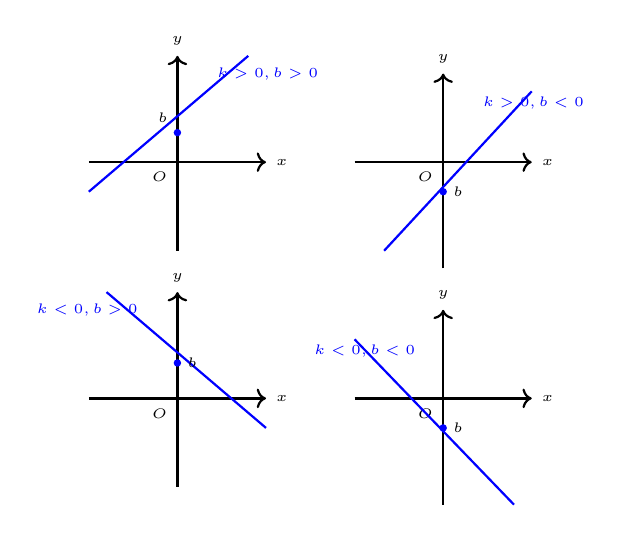
\begin{tikzpicture}[scale=0.75, thick]

  % ====== 左上：k>0, b>0 (一、二、三象限) ======
  \begin{scope}[shift={(-3.5, 2.5)}]
    \draw[->] (-1.5,0) -- (1.5,0) node[right] {\tiny$x$};
    \draw[->] (0,-1.5) -- (0,1.8) node[above] {\tiny$y$};
    \node[below left] at (0,0) {\tiny$O$};
    \draw[blue, thick] (-1.5,-0.5) -- (1.2,1.8);
    \fill[blue] (0,0.5) circle (1.8pt);
    \node[right, blue, font=\tiny] at (0.5,1.5) {$k>0,b>0$};
    \node[above left, font=\tiny] at (0,0.5) {$b$};
  \end{scope}

  % ====== 右上：k>0, b<0 (一、三、四象限) ======
  \begin{scope}[shift={(1.0, 2.5)}]
    \draw[->] (-1.5,0) -- (1.5,0) node[right] {\tiny$x$};
    \draw[->] (0,-1.8) -- (0,1.5) node[above] {\tiny$y$};
    \node[below left] at (0,0) {\tiny$O$};
    \draw[blue, thick] (-1.0,-1.5) -- (1.5,1.2);
    \fill[blue] (0,-0.5) circle (1.8pt);
    \node[right, blue, font=\tiny] at (0.5,1.0) {$k>0,b<0$};
    \node[right, font=\tiny] at (0,-0.5) {$b$};
  \end{scope}

  % ====== 左下：k<0, b>0 (一、二、四象限) ======
  \begin{scope}[shift={(-3.5, -1.5)}]
    \draw[->] (-1.5,0) -- (1.5,0) node[right] {\tiny$x$};
    \draw[->] (0,-1.5) -- (0,1.8) node[above] {\tiny$y$};
    \node[below left] at (0,0) {\tiny$O$};
    \draw[blue, thick] (-1.2,1.8) -- (1.5,-0.5);
    \fill[blue] (0,0.6) circle (1.8pt);
    \node[left, blue, font=\tiny] at (-0.5,1.5) {$k<0,b>0$};
    \node[right, font=\tiny] at (0,0.6) {$b$};
  \end{scope}

  % ====== 右下：k<0, b<0 (二、三、四象限) ======
  \begin{scope}[shift={(1.0, -1.5)}]
    \draw[->] (-1.5,0) -- (1.5,0) node[right] {\tiny$x$};
    \draw[->] (0,-1.8) -- (0,1.5) node[above] {\tiny$y$};
    \node[below left] at (0,0) {\tiny$O$};
    \draw[blue, thick] (-1.5,1.0) -- (1.2,-1.8);
    \fill[blue] (0,-0.5) circle (1.8pt);
    \node[left, blue, font=\tiny] at (-0.3,0.8) {$k<0,b<0$};
    \node[right, font=\tiny] at (0,-0.5) {$b$};
  \end{scope}

\end{tikzpicture}
\end{document}
